\documentclass[12pt,fleqn]{article}\usepackage{../common}
\begin{document}
Ders 19

Eslenik Gradyan (Conjugate Gradient) Yontemi 

Arnoldi metotu Gram-Schmidt'e benzeyen bir yontemdir ve bir ortogonal baz
ortaya cikartir. Bu baz, Krylov altuzayinin bazidir, ki bu altuzaydaki her
yeni baz vektor, $e$'nin baska bir ustu alinip carpilarak elde
edilir. Fakat bu pek iyi bir baz degildir, bazlarin ortogonalize edilmesi
gerekir, ve Arnoldi'nin yaptigi budur.

Arnoldi-Lanczos yontemi ozdegerler (eigenvalue) bulmak icin de kullanilir.

\[ AQ = QH \]

esitligindeki $H$ matrisinin alt-matrisine bakilirsa, aranilan ozdegerler
buradan okunabilir. Bu alt-matris simetrik ve ust kosegendir.
(upperdiagonal). 

\[ H = Q^{-1}AQ \]

formulunde $H,A$ matrisleri birbirine benzerdir (similar) ve benzer
matrislerin ozdegerleri aynidir. 

Bu kavramlardan soyle bir bahsetmek istedim, belki gunun birinde cok buyuk
bir matrisin ozdegerlerini bulmak istersiniz, aklinizda olsun. Yazilim
\verb!arpack! bunun icin kullanilabiliyor. Bahsi yaptik bir diger sebep
lineer cebirin yarisi lineer sistemlerse, diger yarisi ozdeger
problemleridir denebilir. Buraya gelmisken ustteki ozdeger yonteminden
bahsetmemek olmazdi. 

Konumuza donelim. 

$A$ pozitif kesin ve simetrik olmali. Eger degilse birazdan gosgterecegimiz
formulleri kullanmak biraz riskli olur, isleyebilirler ama garanti olmaz. 

$r_K = b - Ax_k $, $K_k$'ye ortogonal, $x_k \in \mathscr{K}_K$. 

Demek ki $x_k$'yi ozyineli olarak yaratabiliriz, ve her adimda sadece $A$
ile carpmamiz gerekir. Ustteki formulde $A$ ile carpim olduguna gore, $r_K$
bir sonraki uzay $k+1$ icinde olacaktir. Arnoldi'den biliyoruz ki $q_{k+1}$
ayni uzay icindedir. O zaman 

$r_k$, $q_{k+1}$'in bir katidir. Yani $r$ ile gosterilen ``artiklar
(residuals)'' birbirine ortogonal. Yani 

\[ r_i^Tr_k = 0, \ i < k \]

Artiklarin birbirine ortogonal olmasinin sebebi iclerinde $A$ olmasi. 

Baslangic degerleri

\[ d_0 = b \]

\[ x_0 = 0 \]

\[ r_0 = b - Ax_0  = b\]

Simetrik Pozitif Kesin $A$ Icin Eslenik Gradyan Metodu

\begin{lstlisting}[language=Matlab,mathescape,numbers=left,xleftmargin=3.0ex]
$\alpha_k = r_{k-1}^T r_{k-1} / d_{k-1}^T A d_{k-1}$
$\alpha_k = \alpha_{k-1} + \alpha_k d_{k-1}$
$r_k = r_{k-1} - \alpha_k Ad_{k-1}$
$\beta_k = r_k^Tr_k / r_{k-1}^Tr_{k-1}$
$d_k = r_k + \beta_k d_{k-1}$
\end{lstlisting}

$d$ ``arama yonudur'', optimizasyon ilerlerken gidecegimiz
istikamettir. 2. adimda guncellemeyi yapiyorum. Peki bir sonraki yonum ne
olmali? 

Her Dongude:

- $Ad$ carpimini goruyoruz, cunku $A$ ile carpim bize yeni Krylov altuzayini
veriyor.\\
- 2 icsel carpim \\
- 2 ya da 3 vektor guncellemesi

Peki $k$ adim sonra hata $||e_k||$ nedir ve ilk bastaki hata $||e_0||$ ile
baglantisi nedir? 

\[ ||e_k|| \le 2  \bigg(
\frac{ \sqrt{ \lambda_{maks} - \lambda_{min}}}
{\lambda_{maks} + \lambda_{min}}
\bigg)^k||e_0||
\]

Hala bir kelimeye aciklik getirmedik; gradyan. Niye bir ``gradyan''
kelimesi kullaniyoruz, neyin gradyanindan bahsediyoruz, bu teknik icin
gradyanlar ne anlama geliyor?

Lineer problemlerde $Ax = b$ esitligi vardir ve bu esitlik enerjinin
gradyanindan gelir. Yani 

\[ E(x) = \frac{ 1}{2}x^TAx - b^Tx \]

enerjisinin gradyanindan. Ustteki formul nereden geldik diye
dusunebilirsiniz, hep lineer sistemlerden bahsettik, ve bu sistemlerde her
sey $Ax = b$ formatina uyar. Simdi birdenbire matematigin farkli bir koluna
geciyorum sanki, ustteki formulu minimize etmeye ugrasiyorum, yani
optimizasyona giriyorum. Fakat cebirsel olarak dusunursek, 

\[ grad \ E = [\frac{\partial E}{\partial x} ]  = Ax - b \]

olacaktir. Minimumda ustteki sifir olacagina gore 

\[ Ax - b = 0 \]

\[ Ax = b \]

Yani karesel enerjinin lineer gradyani vardir, ve onun minimumu $Ax =
b$'dir. 
Bu demektir ki lineer denklemi cozmek ve enerjiyi minimize etmek
aslinda ayni seydir! Minimum kelimesini kullanabiliyorum bu arada, cunku
$A$'nin pozitif kesin oldugunu biliyorum. 

Minimize islemi nasil yapilir? Diyelim ki alttaki gibi bir $E(x)$'im var,
kap seklinin herhangi bir noktasindayim, ve asagi inmem lazim. En fazla
artis gradyan $g$ ise, dibe inmek icin $-g$ yonunde gidebilirim. 

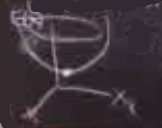
\includegraphics[height=2cm]{19_1.png}

Bu yon dogal bir yondur, ilk akla gelen fikirdir ve mantiklidir. Fakat en
iyi yon degildir. Simdi minimizasyon cozumu olarak eslenik gradyan
acisindan bakiyoruz olaya, isin gradyan tarafi da boylelikle acikliga
kavusacak. 

Negatif gradyanin ayni zamanda artigin da (residual) negatif
yonudur. Artigin yonunde hareket etmek iyi midir? Negatif gradyani takip
etmenin bir diger ismi ``en dik inis (steepest descent)''tir. Fakat,
baslangic noktasina gore bu degisir ama, cok fazla inis cikis ta
yasanabilir.

$r$'ler hesapsal bilimde cok aranan bir ozellige sahip degildir,
ortogonallik. Bir sekilde ortogonallik her zaman dogru yonde hareket
ettigimizin garantisidir. Gidilmesi gereken dogru yon, ustteki kodda
5. satirda hesaplanan yondur. Bu yone ``$A$-ortogonal'' denir. 

Bir resimle gostermek gerekirse, alta bakalim, soldaki en dik inis, sagdaki
eslenik gradyan. Enerji fonksiyonunu kesit seviyesinden (level set), cevrit
(contour) olarak gosteriyoruz, her cevrit bir enerji seviyesine tekabul
edecek, mesela en distaki cevrit 5, bir icerideki 4 olabilir, ve en
ortadaki nokta tam sifir olabilir, cunku en dusuktur. 

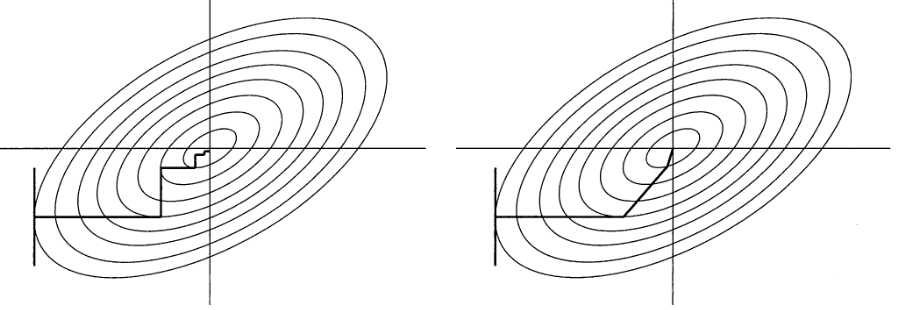
\includegraphics[height=4cm]{19_2.png}

Her iki teknigin gidisati resimde gorulmektedir. 

[gerisi atlandi]

Ekler 

Ustteki anlatimda Krylov altuzaylarinin eslenik gradyan metotunun
isleyisinde tam olarak nasil rol oynadigi belirtilmemis. Aslinda Krylov
altuzaylari gerektirmeden bu metotu anlatmak mumkun. 

Iki vektor $u,v$ birbirine A-ortogonaldir eger

\[ u^TAv = 0 \] 

ise. Dikkat, bu iki vektor, tek baslarina, $u^Tv$ olarak birbirine
ortogonal olmayabilir, ama ortada $A$ oldugu halde carpim sifir cikarsa
ortogonal olmasalar da A-ortogonal olurlar. Bu ortogonalligin bir diger
ismi eslenik (conjugate) olmaktir.

Simdi diyelim ki elimizde herbiri birbirine ortogonal olan $n$ tane
$\{d_k\}$ yonu / vektoru var. O zaman $d_k$ $\mathbb{R}^n$ icin bir baz
olusturur ve biz de $Ax = b$ denkleminin cozumu $x_*$'i bu bazi temel
alarak temsil ederiz. Yani baz vektorlerini carpan bazi katsayilar vardir,
ve bu carpimlarin toplami $x_*$ olur. 

\[ x_* = \sum _{ i=1}^{n} \alpha_i d_i \]

Boylece $Ax = b$'yi cozmek icin bir metot elde ediyoruz, eger $n$ tane
eslenik yon bulabilirsek, $\alpha$ degerlerini hemen hesaplayabiliriz.
Ayrica eger eslenik vektorler $d_k$'leri dikkatlice secersek, yaklasik cozum $x_*$
icin hepsine ihtiyacimiz olmaz. Ozyineli $x$ formulunu kullanabiliriz,

\[ x_{k+1} = x_k + \alpha_k d_{k+1} \ \ \ \label{1} \]

Bu formul niye mantikli? Eger cozum $x_*$ ortogonal $d_k$ vektorlerinin bir
lineer kombinasyonu ise, cozum vektorleri birbiri ardina dizilmis ve ``bir
yere giden'' bir zincir olarak gorulebilir. Ustteki formul sadece bu
zinciri yavas yavas kurmakta..

Ilk once ozyineli olarak artiklar $r_k$ arasinda bir iliski kuralim,
(1)'nin iki tarafi $A$ ile carpip, $b$'den cikartalim (cunku
$r_i = b -
Ax_i$'a erismek istiyoruz),

\[b - A x_{k+1} = b - A x_k  + \alpha_k A d_{k} \]

\[r_{k+1} = r_k + \alpha_k A d_{k} \]

\[r_{k+1} = r_k + \alpha_k A d_{k} 
\ \ \ \label{8}
\]

Simdi hata terimini hesaplayalim. $e_i$, yani $i$'inci tahminin hatasi, 

\[ e_i = x - x_i  \]

Iki tarafi $A$ ile carpalim

\[ Ae_i = Ax - Ax_i  \]

\[ Ae_i = b - Ax_i  \]

Sag taraf $r_i$ taniminin aynisi degil mi? O zaman 

\[ Ae_i = r_i 
\ \ \ \label{5}
\]

$e$'yi ozyineli olarak temsil etmek te mumkundur, (1)'nin her iki
tarafindan $x$ cikartirsam, 

\[ x_{k+1} - x = x_k - x + \alpha_k d_{k} \]

\[ e_{k+1} = e_k + \alpha_k d_k \ \ \ \label{2}\]

Bu her adimi $\alpha_k$'ye bagli ozyineli bir tanimdir. 

$\alpha$ katsayilarini bulmak icin bir sonraki yonden gelen hatanin onceki
tum arama yonlerine, ozelde bir onceki arama yonune A-ortogonal
olmasini istiyoruz. Yani

\[ d_i^TA e_{i+1}  = 0\]

olmali. 

\[ d_i^TA (x_{i+1}-x)  = 0\]

\[ d_i^TA (x_{i} + \alpha_i d_i -x)  = 0\]

\[ d_i^TA (e_i + \alpha_i d_i )  = 0\]

\[ d_i^Tr_i + \alpha_i d_i^TA d_i   = 0\]

\[ \alpha_i = -\frac{ d_i^Tr_i}{d_i^T A d_i} 
\ \ \ \label{6}
\]

Simdi hata terimine donelim, diyelim ki $e_0$ vektoru, bu vektor, diger
her vektor gibi icinde oldugumuz uzayin bazlarinin bir kombinasyonu olarak
temsil edilebilir. Bizim bazlarimiz $d_j$ olduguna gore, 

\[ e_0 = \sum _{ j=0}^{n-1} \delta_j d_j \]

Katsayi olarak $\delta_j$ sectik, $\alpha$ ile karisiklik olmasin
diye. Simdi iki tarafi $d_k^T A$ ile carpalim, 

\[ d_k^T A e_0 = \sum _{ j=0}^{n-1} \delta_j d_k^T A d_j \]

Yine ayni ortogonallik numarasi, toplam icinde $j$ olmayan tum diger $p$
carpimlari sifirdir, 

\[ d_k^T A e_0 =  \delta_j d_j^T A d_j \]

\[ \delta_j = \frac{ d_k^T A e_0}{ d_j^T A d_j } 
\ \ \ \label{4}
\]

Simdi $e_0$'in yerine (2)'teki ozyineli tanimdan turetecegim bir sey koymak
istiyorum. Diyelim ki $e_0$'dan baslayip teker teker bir sonraki $e$'yi
hesaplayip alt alta yazdim, ve topladim

\[ \cancel{e_{1}} = e_0 + \alpha_0 d_0\]

\[ \cancel{e_{2}} = \cancel{e_1} + \alpha_1 d_1\]

\[ ... \]

\[ e_{k} = \cancel{e_{k-1}} + \alpha_{k-1} d_{k-1}\]


Sag kalan tek terimler 

\[ e_k = e_0 + \sum _{ j=0}^{k-1} \alpha_j d_j \]

(4) icinde $e_0$ yerine koyalim

\[ \delta_j = \frac{ d_k^T A e_k - \cancel{\sum _{ j=0}^{k-1} \alpha_j d_k^T A d_j}}
{ d_j^T A d_j } 
\]

Niye iptal? Yine A-ortogonalligi. Dikkat edilirse $j$'ler $k-1$'e kadar
cikiyor, $k$'ye bile erismiyor, carpim hep sifir. Kalanlar,

\[  = \frac{ d_k^T A e_k}
{ d_j^T A d_j } 
\]

(5)'i kullanirsak, 

\[ \delta_j = \frac{ d_k^T r_k}
{ d_j^T A d_j } 
\]


(6) ile bu formulun benzerligi bariz, sadece eksi isareti farkli. O zaman 

\[ \delta_k = -\alpha_k \]

diyebiliriz. Bu demektir ki hata formulunde $\alpha$ yerine $\delta$
kullanabiliriz, 

\[ e_0 = -\sum _{ j=0}^{n-1} \alpha_j d_j \]

Hatalarin ozyineli denklemi (2)'yi uste uygularsak, 

\[ e_i = -\sum _{ j=i}^{n-1} \alpha_j d_j 
\ \ \ \label{3}
\]

Simdi artiklarin ve onceki gidis yonlerinin ortogonal olduklarini
gosterelim. (3)'u $d_k^TA$ ile carpalim, 

\[ d_k^TAe_i = -\sum _{ j=i}^{n-1} \alpha_j  d_k^TAd_j 
\]

\[ d_k^Tr_i = -\sum _{ j=i}^{n-1} \alpha_j  d_k^TAd_j 
\]

$d$'ler arasindaki A-ortogonallik sayesinde ve $k < i$ icin 

\[ d_k^Tr_i = 0
\ \ \ \label{9}
\]

Madem ki eski yonler ve artiklar birbirine ortogonal, Gram-Schmidt
isleminin A-ortogonal halini artiklardan yon uretmek icin
kullanabiliriz. Her artigi alip, icinden ona ortogonal bir yon cikartmak
mumkun.

\[ d_i = r_i + \sum _{ j=0}^{i-1} \beta_{i,j}d_j 
\ \ \ \label{10}
\]

\[ \beta_{i,j} = - \frac{ r_i^TAd_j}{d_j^TAd_j} \]

Yani Gram-Schmidt formulasyonunun A-ortogonallik kullanan hali (bkz Lineer
Cebir Ders 17 notlari). Ama ustteki ifadeyi daha da basitlestirebiliriz, ve
verimli hale getirebiliriz. Ustteki yontemde tum vektorleri etrafta
tutmamiz gerekiyor, ayrica $A$'lardan kurtulmak iyi olur. 

Kurtulmak icin $r_i^TAd_j$ ifadesine icinde ulasmaya calisacagiz, ve
esitligin diger tarafinda icinde $A$ olmayan bir ifade olmasina gayret
gosterecegiz. $r_i^Tr_{j+1}$ ile baslayalim, ve $r_{j+1}$ uzerinde ozyineli
denklem (8)'i uygulayalim. 

\[ r_i^Tr_{j+1} = r_i^T (r_i + \alpha_k A d_k)  = r_i^Tr_j + \alpha_i r_i^TAd_j \]

\[ = \frac{ r_i^Tr_{j+1} - r_i^Tr_j }{\alpha_j} =  r_i^TAd_j \]

Esitligin sagindaki ifadenin $\beta_{i,j}$ ifadesinin bolunen kismi ile
ayni olduguna dikkat, ve esitligin sol tarafinda $A$ yok. Yerine koyalim, 

\[ \beta_{i,j} = - \frac{ 1}{\alpha_j}\frac{  r_i^Tr_{j+1} - r_i^Tr_j }{d_j^TAd_j} \]

$j = i -1$, yani $\beta_{i,i-1}$ icin

\[ \beta_{i,i-1} = - \frac{ 1}{\alpha_{j-1}}\frac{  r_i^Tr_i  }{d_{i-1}^TAd_{i-1}} \]

$r_i^Tr_j$ terimi $r_i^Tr_{i-1}$ olunca sifir oldu, cunku artiklar birbirine ortogonal. 
Dikkat bu sefer ortogonal, A-ortogonal degil. Bunu nasil ispat ederiz? 
(10)'u alip $r_k$ ile carpalim, ve $k,i$ indislerini degistirelim

\[ d_k^Tr_i = r_k^Tr_i + \sum _{ j=0}^{i-1} \beta_{k,j}d_j ^Tr_i = 0
\]

Sifira esitlik (9) sayesinde. Ama bu sifir durumu toplam icindekiler icin
de gecerli, cunku toplamin ust siniri $i-1$, ve en yuksek indisli yon
$d_{j-1}$ olabilir, o zaman toplam da sifirdir. Yani

\[  r_k^Tr_i  = 0 \]

$\beta$ ile isimize devam edelim. Bolen kisminda hala bir $A$ var, onu
yokedelim. Once (6)'daki $\alpha$ taniminin $i-1$ indisli haline bakalim, ve
tersine cevirelim, 

\[ \frac{ 1}{\alpha_{i-1}} = -\frac{d_{i-1}^T A d_{i-1} }{d_{i-1}^Tr_{i-1}} 
\]

Son $\beta$ formulunde yerine koyalim

\[ \beta_{i,i-1} = 
\frac{  r_i^Tr_i  }{ \cancel{d_{i-1}^TAd_{i-1}}} 
\frac{\cancel{d_{i-1}^T A d_{i-1}}}{d_{i-1}^Tr_{i-1}}
= 
\frac{  r_i^Tr_i  }{d_{i-1}^Tr_{i-1}}
\]


Son bir esitlik daha var, bu da $d_{i-1} = r_{i-1}$ esitligi, nereden
geliyor?  $j < i-1$ icin $r_i^Tr_{j+1}$ ve $r_i^Tr_{j}$ carpimlarinin ikisi
de sifirdir, o zaman (10) formulu

\[ d_i = r_i + \beta_{i,j}d_j \]

haline gelir cunku pek cok deger icin $\beta_{i,j} = 0$ olacaktir. Simdi
usttekini bir onceki indis degerleri icin tekrar yazalim,

\[ d_{i-1} = r_{i-1} + \beta_{i-1,i-2}d_{i-2} \]

Yine ortogonallik sayesinde $\beta$ degeri iptal olur, ve geriye sadece 

\[ d_{i-1} = r_{i-1} \]

kalir. Boylece son formul

\[ \beta_{i,i-1} = 
\frac{  r_i^Tr_i  }{r_{i-1}^Tr_{i-1}}
\]

haline geliyor, ve kodlama cok temizlesiyor. 

\lstinputlisting[language=Python]{cg.py}


\end{document}
